

\section{Co-residence Detector for Lambdas}
\label{sec:methodology}

% TODO: This figure shows only mem access latencies of exotic 
% operation. how does these operations affect latencies of other exotic 
% operations or regular memory accesses?
\begin{figure*}[h!]
\begin{subfigure}{.33\textwidth}
  \centering
  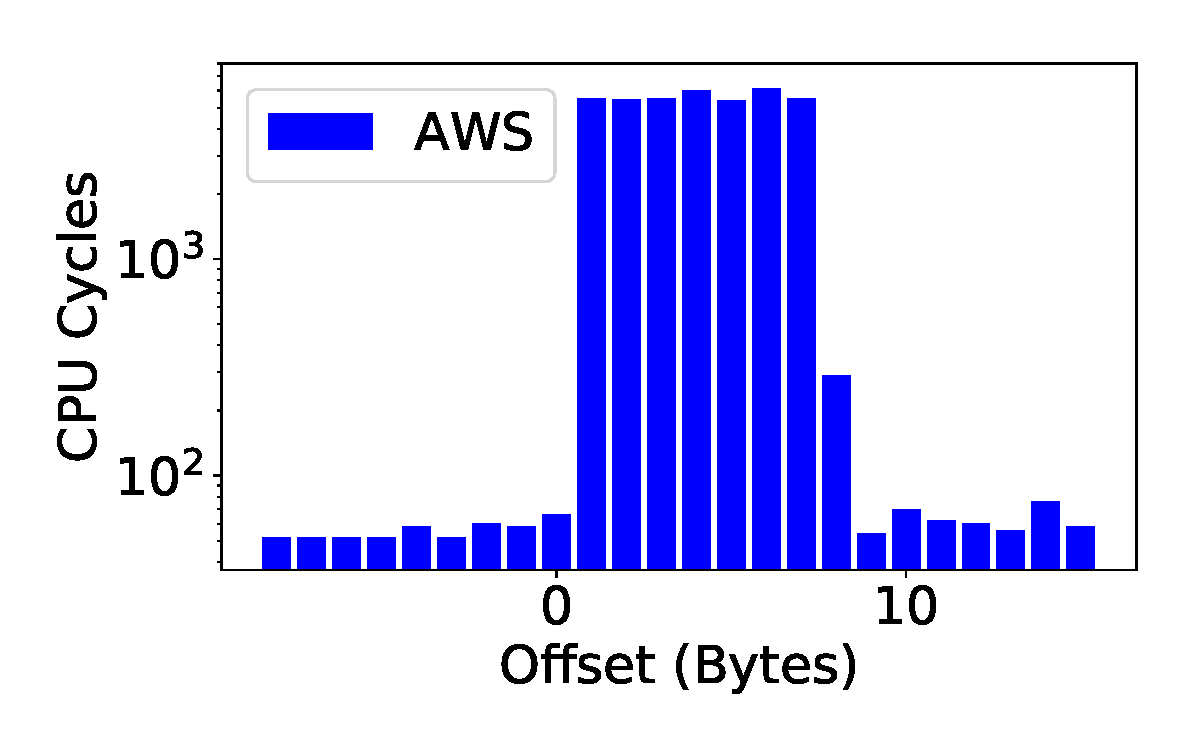
\includegraphics[width=.99\linewidth]{fig/membus_aws.pdf}
%   \caption{1a}
%   \label{fig:sfig1}
\end{subfigure}%
\begin{subfigure}{.33\textwidth}
  \centering
  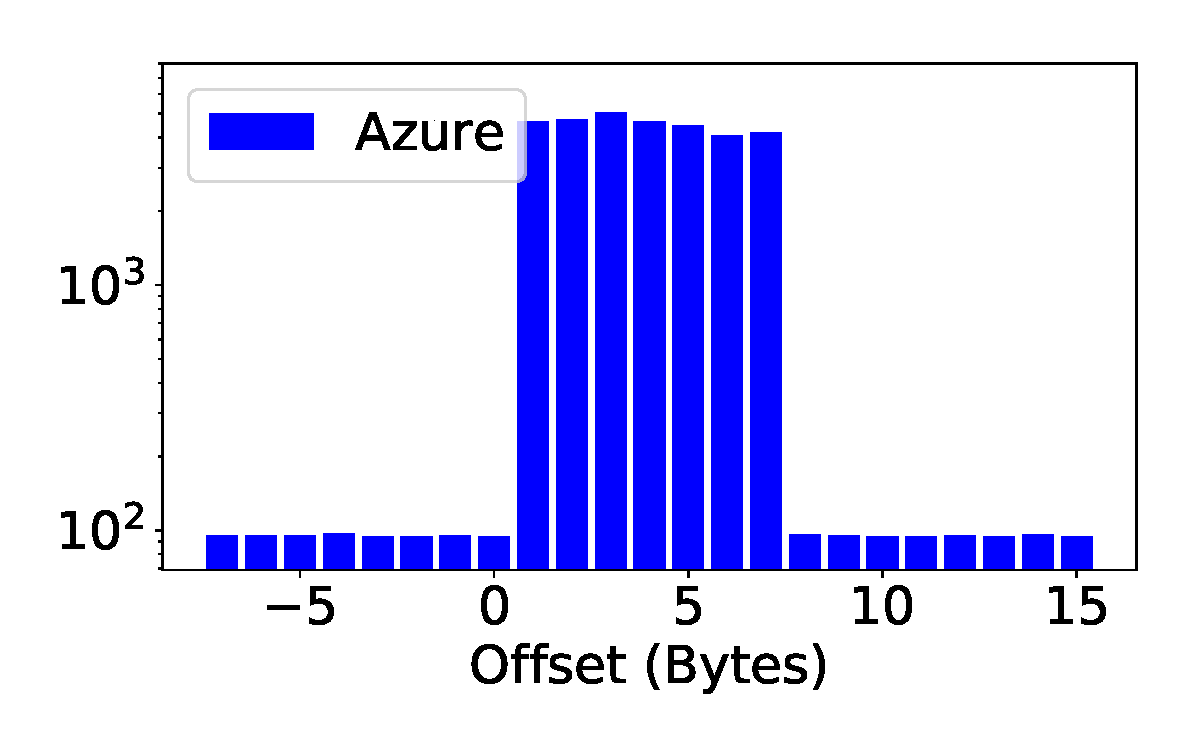
\includegraphics[width=.99\linewidth]{fig/membus_azure.pdf}
%   \caption{1b}
%   \label{fig:sfig2}
\end{subfigure}
\begin{subfigure}{.33\textwidth}
  \centering
  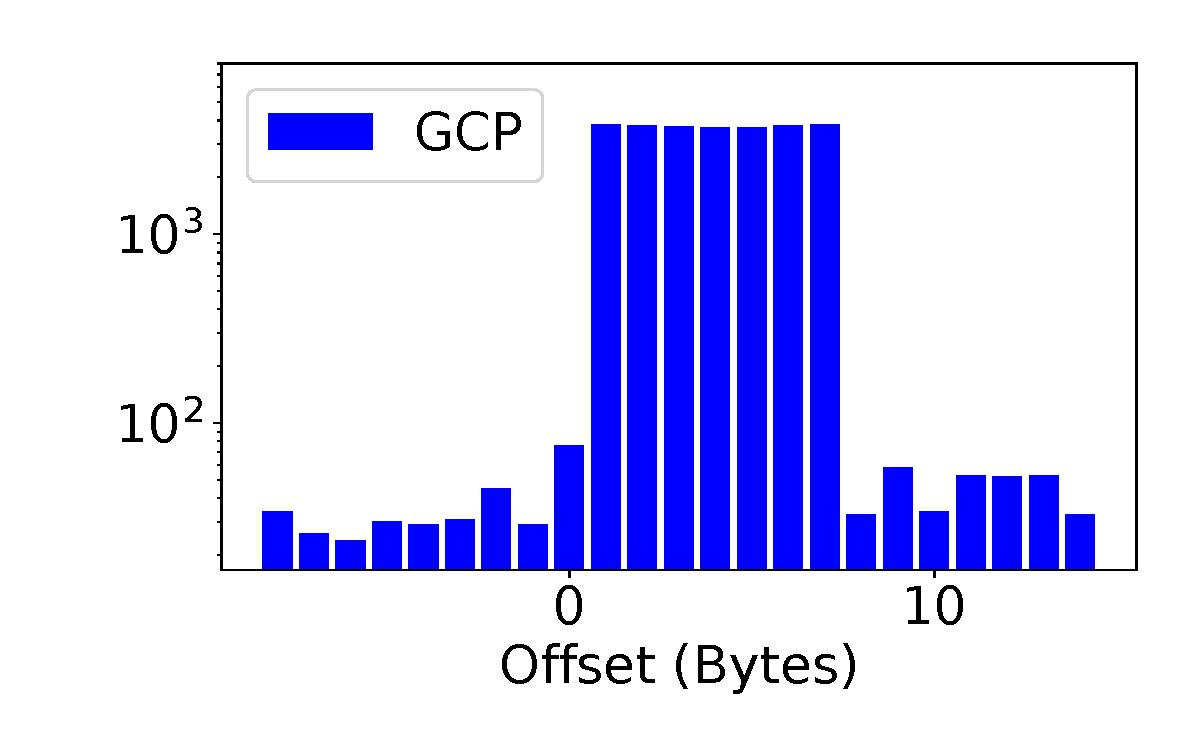
\includegraphics[width=.99\linewidth]{fig/membus_gcp.pdf}
%   \caption{1b}
%   \label{fig:sfig2}
\end{subfigure}
\caption{The plots show the latencies of atomic memory operations performed on
        an 8B memory region as we slide from one cache line across the boundary into
        another on AWS, Azure, and Google (GCP) respectively.  The latencies are orders
        of magnitude higher when the 8B region falls across the two cache lines (offsets
        0-7B), demonstrating the presence of the memory bus covert channel on all these
        cloud providers. \label{fig:membus_clouds}}
\label{fig:fig}
\end{figure*}


In this section, we present a novel co-residence detector for lambdas, previous 
solutions to this problem, and the unique challenges we faced with lambdas and
how we address each of them.

\subsection{Specification}
Given a set of cloud instances (VMs, Containers, Functions, etc) deployed to a
public cloud, a co-residence detection mechanism should identify, for each pair
of instances in the set, whether the pair is running on the same physical
server at some point. Paraphrasing Varadarajan et al.~\cite{varadarajan2015},
for any such mechanism to be useful across a wide range of launch strategies, it
should have the following properties:

\begin{itemize}
    \item \textbf{Generic} The technique should be applicable across a wide
    range of server architectures and software runtimes. In practice, the
    technique would work across most third-party cloud platforms and even 
    among different platforms within a cloud.
    \item \textbf{Reliable} The technique should have a reasonable detection success
    with minimal false negatives (co-resident instances not detected) and even 
    less false positives (non co-resident instances categorized as co-resident).
    \item \textbf{Scalable} A launch strategy may require hundreds or even
    thousands of instances to be deployed, and must scale such that the
    technique will detect all co-resident pairs at a reasonable cost.
\end{itemize}

\noindent We add another property to that list which is relevant to lambdas:
\begin{itemize}
    \item \textbf{Fast} The technique should be fast, preferably finishing in 
    the order of seconds. As lambdas are ephemeral (with some clouds restricting their 
    execution times to as low as a minute), the technique should leave ample time 
    for other activities that make use of the resulting co-resident information.
\end{itemize}


\subsection{Design}

\subsubsection{Using Covert Channels for Generality}
As mentioned in section \ref{sec:background:coresidence}, co-residence detection 
was previouly done using unique software idenitifers that revealed underlying server 
to the tenants. Such software identifiers present the fastest and perhaps most 
reliable(\anil{reliable as in trustworthy information}) way for co-residence detection 
as all it takes is for each lambda to quickly
"read" the identifier and communicate this information with all other lambdas 
(through the network or shared remote storage) to identify the 
neighbors. However, such information can be easily obfuscated by platform providers;
for example, currently there is no such identifier available for AWS lambdas. 
So we turn to hardware-based covert channels that are, by definition, also accessible to all the 
tenants. They are also generally more difficult to remove, and more pervasive too, 
given that hardware is more homogenous across computing platforms than software. 
%We discuss our use of
%hardware-based covert channels and how producing a reliable and scalable
%mechanism also fulfills the need for a generic and fast protocol.


\subsubsection{Covert Channels Cannot Support Multiple Parties}
\todo{think about this paragraph}
As covert channels can send information, naturally we can expect to use the 
channel to communicate identity information (like unique ids) between 
co-resident lambdas all of which have access to the channel. However,
covert channels generally presume that the sender and the receiver are 
already known and that there will be only two parties performing 
communication. But when multiple parties share a channel, we would need 
a channel access control, such as MAC protocols in Ethernet networks, 
to arbitrate access to the channel and handle collisions as they 
are in the same collision domain. However, covert channels are often 
binary channels (i.e., parties can either only send or receive a bit 
but not both) with no capability for collision detection and have very 
limited bandwidth (often only tens of bits per second) that such 
channel arbitration can be infeasible or complex enough to present 
significant overhead on channel bandwidth. 



\subsubsection{A fast ID broadcast designed for covert channels}
\label{sec:method:protocol}


\begin{algorithm}[!t]
\caption{Neighbor discovery protocol}
\label{alg:protcol}
\begin{algorithmic}[1]
\STATE $sync\_point \leftarrow$ {Start time for all instances}
\STATE $ID \leftarrow$ {Instance ID}
\STATE $N \leftarrow$ {Number of bits in ID}
\STATE $advertising \leftarrow TRUE$
\STATE $instances \leftarrow \{\} $
\STATE $WAIT\_TILL(sync\_point)$
\WHILE{$id\_read$}
    \STATE $slots \leftarrow 0$
    \STATE $id\_read \leftarrow 0$
    \STATE $participating \leftarrow advertising$
    \WHILE{$slots < N$}
        \STATE $bit \leftarrow$ {$slots^{th}$ most significant bit of ID}
        \IF{$participating$ \textbf{and} $bit$}
            \STATE $WRITE\_BIT()$               (Alg. \ref{alg:sender})
            \STATE $bit\_read \leftarrow 1$
        \ELSE
            \STATE $bit\_read \leftarrow READ\_BIT()$       (Alg. \ref{alg:receiver})
            \IF{$bit\_read$}
                \STATE $participating \leftarrow FALSE$
            \ENDIF
        \ENDIF
        \STATE $id\_read \leftarrow 2 * id\_read + bit\_read$
        \STATE $slots \leftarrow slots + 1$
    \ENDWHILE
    \IF{$id\_read = ID$}
        \STATE $advertising \leftarrow FALSE$
    \ENDIF
    \STATE $instances \leftarrow instances \cup \{id\_read\}$
\ENDWHILE
\STATE \textbf{return} $instances$
\end{algorithmic}
\end{algorithm}

For co-residence detection, lambdas only need to communicate their IDs with one another
and as such, we don't need the channel to be very general and expressive. 
Thus, we assume that each lambda involved has a unique fixed-length (say \emph{N}) 
bit-string corresponding to its ID that must be communicated.  
In regards to the covert channel, we only assume that any lambda with access to the 
channel can choose to either send or listen for a bit, and if at least one lambda 
chooses to send a 1-bit, all the listeners would record a 1-bit. 
We also assume that lambdas can synchronize themselves between sending or listening 
a bit in each time slot. We show both these assumptions to be reasonable in 
section \ref{sec:method:impl}. 
As such, we propose a communication protocol that efficiently broadcasts 
just these bit-strings on channels with such restricted properties.

We divide the total running time of the protocol into phases, with each phase executing for an
interval of \textit{N} bit-slots. Each phase has a set of \textit{participating}
lambdas, which in the first phase would be all of the lambdas. In
each bit-slot \textit{K} of \textit{N} slots in a phase, every participating
lambda broadcasts a bit if the $K^{th}$ bit of its bit-string (ID) is 1,
otherwise it listens for a 0 or 1. If an lambda senses a 1 while listening, it
stops participating, and listens for the rest of the phase. Thus, only the
lambdas with the highest ID among the initial set of participating lambdas
continues broadcasting until the end of the protocol, effectively advertising
its full ID to the rest of the (now listening) lambdas. In the next phase, the
lambda with the previously highest ID now only listens, allowing the next
highest lambda to advertise its ID, and so on.  If the IDs are unique,
there will always be only one lambda that broadcasts in every phase. The
protocol ends after \textit{x} phases (where \textit{x} is number of co-resident
lambdas), when none of the lambdas broadcast for \textit{N} consecutive
bit-slots. The pseudo-code of the protocol is provided in Algorithm
\ref{alg:protcol}. 
%Note that the protocol itself is channel-agnostic and can be
%extended for other (future) covert channels with similar channel properties.

% Figure moved here for formatting
\begin{figure}[!t]
  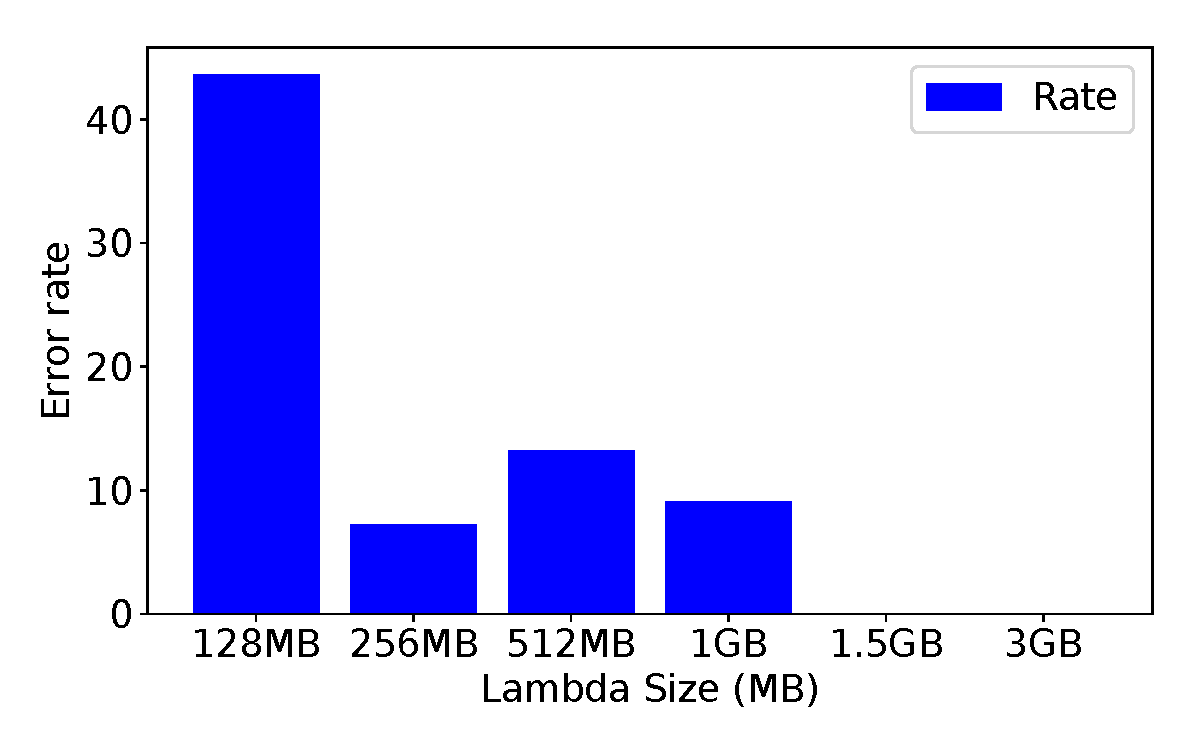
\includegraphics[width=.99\linewidth]{fig/errorrates.pdf}
  \caption{This figure presents the error rate (as a fraction of 1000 lambdas
  deployed) for different lambda sizes in the AWS Middle-East region.
\label{fig:errorrates}}
\end{figure}

\subsubsection{Time Complexity}
\label{sec:protocol:complexity}
Assuming \textit{N} total deployed lambdas to the cloud, the bit-string needs
to be $\log_2N$ bits to uniquely identify each lambda. If a maximum \textit{K}
of those lambdas are launched on the same server, the protocol executes for
\textit{K} phases of $\log_2N$ bit-slots each, taking $(K+1)*\log_2N$ bit-slots
for the whole operation.  In fact, it is not necessary to run the protocol for all \textit{K}
phases. After the first phase, all the co-resident lambdas would know one of
their neighbors (as each phase reveals the ID of the biggest participating
lambda to others).  If we use IDs that are globally unique, all the
co-resident lambdas will see the same ID. The lambdas can then exchange these IDs
offline (e.g., through the network) to infer the rest of their neighbors. This
simplification removes the dependency on number of co-resident lambdas
(\textit{K}) and decreases the complexity to $O(\log_2N)$.

% For example, assuming 10,000 deployed lambdas and a
% maximum of 10 co-resident lambdas on each server, the entire  co-residence
% detection requires around four minutes to fully execute (with 1-second time
% slots).
% allowing the entire
% protocol to finish within a minute instead of four.



\subsection{Implementation}
\label{sec:method:impl}
We implemented the above protocol using a covert channel based on memory bus hardware 
that is available for lambdas. We show how we used the hardware to reliably send and 
listen for bits in order to meet the requirements for the protocol. 

\subsubsection{Introducing Memory Bus Covert Channel}
We utilize the memory bus covert channel described in
section~\ref{sec:background:covertchannels} as it exploits a fundamental
hardware vulnerability that is present across all generations of x86 hardware.
Historically, multiple public cloud services have been vulnerable to this
channel~\cite{varad191016,zhang2016}, and we find that they are still
vulnerable today. To demonstrate the presence of the vuln erability, we measure
the latency of atomic operations on a 8B memory region as we slide the region
from one cacheline into another across the cacheline boundary. We perform this
experiment on three major cloud platforms (AWS, Google and Microsoft Azure) and
show the latencies observed in Figure~\ref{fig:membus_clouds}. From the figure,
we can see that all three cloud platforms still exhibit a significant difference
in latencies for the "exotic" memory locking operations where the memory region
falls across cacheline boundary. When compared to regular memory accesses,
it demonstrates the presence of this covert channel on all of them. Moreover, we
were able to execute these experiments on serverless function instances. Since
lambdas have runtimes that are generally restricted to high-level languages
(that prevent the pointer arithmetic required to perform these exotic
operations), we used the unsafe environments on these clouds --- C++ on AWS,
Unsafe Go on GCP, Unsafe C\# On Azure. This shows the applicability of using the
covert channel across different kinds of cloud instances as well.

\begin{algorithm}[!t]
\caption{Writing 1-bit from the sender}
\label{alg:sender}
\begin{algorithmic}
\STATE $now \leftarrow  time.now()$
\STATE $end \leftarrow now + sampling\_duration$
\STATE $address \leftarrow cache\_line\_boundary-2$
\WHILE{$now < end$}
    \STATE $\_\_ATOMIC\_FETCH\_ADD(address)$
    \STATE $now \leftarrow  time.now()$
\ENDWHILE
\end{algorithmic}
\end{algorithm}

\subsubsection{Sending a bit}
%First, we must determine how to reliably transmit information between the sender and receiver. 
Senders and receivers can accurately communicate 0-bits and 1-bits
by causing contention on the memory bus. To communicate a 1-bit, the sender 
instance causes contention on the memory bus by locking it using the special memory locking operations
(discussed in section~\ref{sec:background:covertchannels}). 
Pseudo-code for the sender instance is shown in Algorithm~\ref{alg:sender}.

\subsubsection{Listening for a bit}
The receiver can simply sample the memory bus for contention, inferring whether 
the communication is a 1-bit (when contention is observed) or a 0-bit 
(when contention is not observed). There are two ways to listen for contetion. 
When the memory bus is locked, any
non-cached memory accesses will queue and therefore see higher latencies.  The
receiver can then continually make un-cached memory accesses (referred to as the
\textit{memory probing} receiver in previous literature~\cite{varadarajan2015})
and observe a spike in their latencies to detect contention. On the other hand,
the receiver can also detect memory bus contention by using the same memory
locking operations as the sender (referred to as \textit{memory locking}
receiver) to probe the memory bus. Since only one processor core can lock the
memory bus at a given time, any other concurrent locking operation will see
higher latency. 

\textbf{Mechanism} Of these two methods, we decide to use the memory locking receiver for our
experiments.  
%Previous studies~\cite{wuusenix2012,varadarajan2015} have
%established that both memory probing and memory locking receivers experience
%significant latency overhead during memory bus contention, making them both
%viable avenues for sensing the covert-channel. 
Since memory probing involves regular (un-cached) memory accesses, it can be done
on multiple receivers concurrently without affecting each other (due to the high
memory bandwidth), which prevents noise in measurements. This is an important
attribute, as memory locking receivers must contend with this noise. However,
bypassing multi-levels of caches in today's servers to perform memory accesses
with reliable consistency is a challenging task. Even with a reliable
cache-bypassing technique, the variety of cache architectures and sizes that we
encounter on different clouds would make tuning the technique to suit these
architectures an arduous task while reducing the applicability of our overall
co-residence detection mechanism. 
%Thus, we decide to use the memory locking receiver as our sensing mechanism.
%% we already said it at the beginning of the paragraph


\begin{algorithm}[!t]
\caption{Reading a bit in the receiver}
\label{alg:receiver}
\begin{algorithmic}[1]
\STATE $now \leftarrow  time.now()$
\STATE $end \leftarrow now + sampling\_duration$
\STATE $sampling\_rate \leftarrow num\_samples / sampling\_duration$
\STATE $address \leftarrow cache\_line\_boundary-2$
\STATE $samples \leftarrow \{\} $
\WHILE{$now < end$}
    \STATE $before \leftarrow RDTSC()$
    \STATE $\_\_ATOMIC\_FETCH\_ADD(address)$
    \STATE $after \leftarrow RDTSC()$
    \STATE $samples \leftarrow samples \cup \{(after-before)\}$
    \STATE \textbf{wait until} $NEXT\_POISSON(sampling\_rate)$
    \STATE $now \leftarrow  time.now()$
\ENDWHILE
\STATE $ks\_val \leftarrow KOLMOGOROV\_SMIRINOV(samples, baseline)$
\STATE \textbf{return} $ks\_val < ksvalue\_threshold$
\end{algorithmic}
\end{algorithm}


\textbf{Sampling frequency}
\label{sec:method:listen:freq}
Another challenge for our protocol is determining an adequate sampling
frequency. Ideally, a memory locking receiver would loop locking operations and
determine contention in real-time by identifying a decrease in the moving
average of the number of operations. Note that, in this case, there is
essentially no difference between the sender and receiver (i.e., both
continually issue locking operations) except that the receiver is taking
measurements. This is adequate when there is a single sender and
receiver~\cite{varadarajan2015}, but when there are multiple receivers, the mere
act of sensing the channel by one receiver causes contention and other receivers
cannot differentiate between a silent (0-bit) and a locking (1-bit) sender. To
avoid this, we space the sampling of memory bus such that no two receivers would
sample the bus at the same time, with high probability. We achieve this by
using large intervals between successive samples and a poisson-sampling to
prevent time-locking of receivers. We determined that a millisecond poisson gap
between samples is reasonable to minimize noise due to collisions in receiver
sampling~\ref{fig:membus_clouds}, assuming ten co-resident receivers and a few
microsecond sampling time. \todo{R1 needed clarification}

\textbf{Sample Size} 
\label{sec:method:samplingdur}
In addition to adequate sampling frequency, we must also determine sample size.  
A receiver can confirm contention with high confidence with only a
few samples, assuming that the sender is actively causing contention on the
memory bus and the receiver is constantly sampling the memory bus throughout the
sampling duration. However the time-sharing of processors
produces difficulties. The sender is not continually causing contention, and
neither is the receiver sensing it, as they are context-switched by the
scheduler, which runs other processes. Assuming that the sender and receiver are
running on different cores, the amount of time they are actively communicating
depends on the proportion of time they are allocated on each core and how they
are scheduled. 

To illustrate such behavior, we run a sender-receiver pair using
lambdas~\cite{awslambda} of various sizes on AWS, and compare the distribution
of latencies seen by the receiver during the contention in each case.
Figure~\ref{fig:context_switching} shows that the much smaller 128 MB lambdas
(which probably share a CPU core and are thus context-switched) exhibit less
active communication than the bigger 3 GB lambdas (which may run on dedicated
cores). This means that smaller instances that tend to share processor cores
with many other instances may need to pause for more time and collect more
samples to make up for lost communication due to scheduling.
% Since the typical scheduling quantum is on the order of milliseconds, they 
% will need at least a second?


\begin{figure}[!t]
  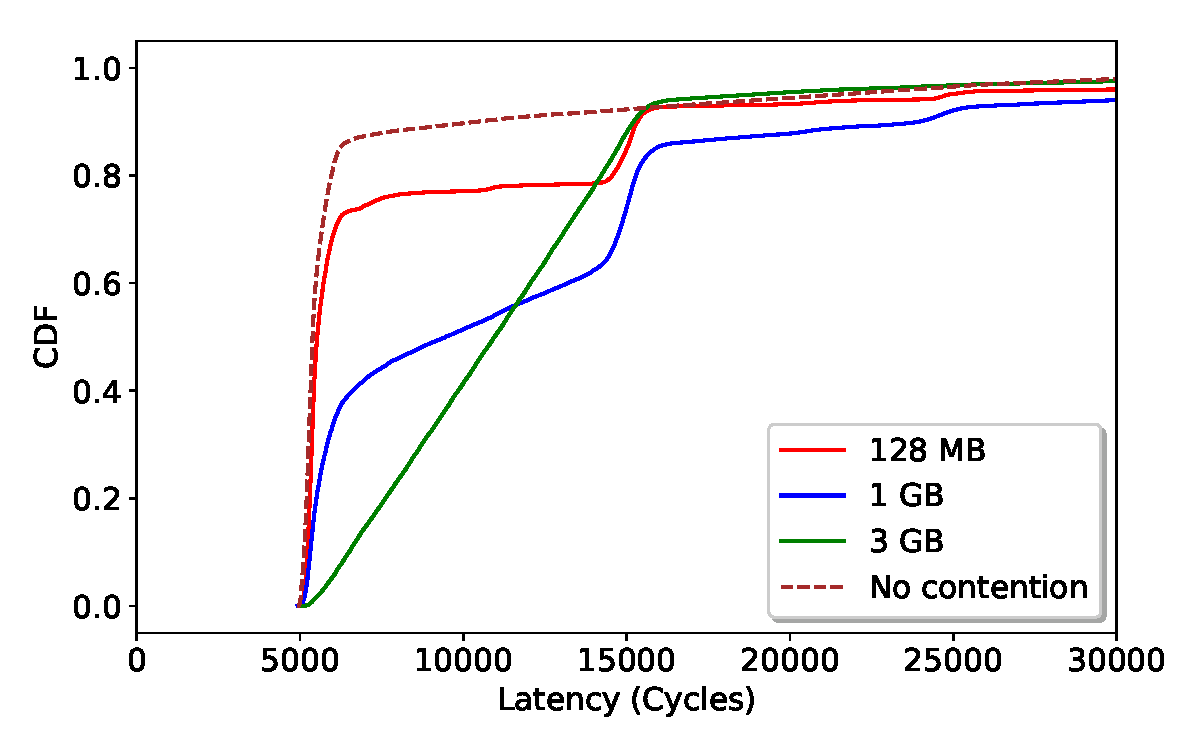
\includegraphics[width=.99\linewidth]{fig/lambda_sched_effect.pdf}
  \caption{We present a CDF of latencies observed by 128 MB, 1 GB and 3 GB
  Lambdas during contention. The 128 MB lambda pair sees less contention due to
  more context switching, whereas the 1 GB and 3 GB lambdas see progressively
  more contention compared to the baseline, which we attribute to their relative
  stability on the underlying physical cores.
\label{fig:context_switching}}
\end{figure}

\textbf{Overcoming noise} 
\label{sec:method:noise}
Along with context switching and sensing noise, there are other imperfections in
the measurement apparatus that may cause noise. For example, we use the
difference in readings from the timestamp counter of the processor (RDTSC)
before and after the locking operation to measure the latency of the operation
in cycles. If the receiver process is context-switched in between the timer
readings (e.g., at line eight in Algorithm~\ref{alg:receiver}), the latency
measured from their difference will be orders of magnitude higher as it includes
the waiting time of the receiver process in the scheduler queue - which we
believe is what contributes to the long tail in
Figure~\ref{fig:context_switching}. To overcome missed samples and noise, we
record hundreds of samples and compare it to the baseline distribution of
latencies sampled without contention. We then need to compare and differentiate
the observed sample of latencies from the baseline to establish contention. To
do this, we use a variant of the two-sample Kolomogorov-Smirinov (KS) test,
which typically compares the maximum of the absolute difference between
empirical CDFs of samples (in our variant, we take the \emph{mean} of the
absolute difference instead of the maximum to reduce sensitivity to outliers). 
Using this measure, we can categorize a KS-value above a certain threshold as a 1-bit
(contention) and a value below the threshold as 0-bit (baseline).

To determine the KS-threshold, we deploy a large number of lambdas across AWS
regions. Some of these lambdas cause contention (aka senders) while others
observe contention by collecting samples of latencies (aka receivers). Each of
the samples may or may not have observed contention depending on whether the
receiver was co-resident with a sender lambda (an unknown at this point). We then
calculate the KS-value for each sample against the baseline and plot a CDF of
these values for lambdas of different sizes in Figure~\ref{fig:ks_values}.
Ideally, we expect a bimodal distribution (stepped CDF) with the upper and
lower peaks corresponding to samples that have and have not seen contention, and
a big gap between the two (long step). Fortunately, we observe this
differentiation with larger lambda sizes (which allows us to choose a clear
threshold), but we do not observe a clear differentiation with smaller lambdas,
where scheduling instability causes lossy communication (discussed
in~\ref{sec:method:samplingdur}).  This trend also reflects in the reliability
of our technique across various lambda sizes, as we will show in our evaluation.
Based on the plot, we picked a KS-threshold at 3.0 which seems to be consistent
across AWS regions, suggesting that this threshold is a platform constant.

We present the pseudo-code of a receiver lambda in Algorithm~\ref{alg:receiver},
which includes all the challenges and subsequent solutions discussed thus
far.

\subsubsection{Synchronization} 
A major enabler of our protocol in section \ref{sec:method:protocol} is the ability 
to synchronize all the co-resident lambdas when sending and receiving 
bits. As all these lambdas are running on the same physical
server, they share the server's clock. On AWS, for example, we observe that the
system clock on lambdas is precise up to nanoseconds. 
Assuming that clocks between different lambdas only exhibit a drift in the order
of microseconds, sampling at a millisecond scale should provide us a margin for
synchronization mismatch. Since we do not observe any synchronization-related
noise in our results, we believe that this is a reasonable assumption.


\begin{figure}[!t]
  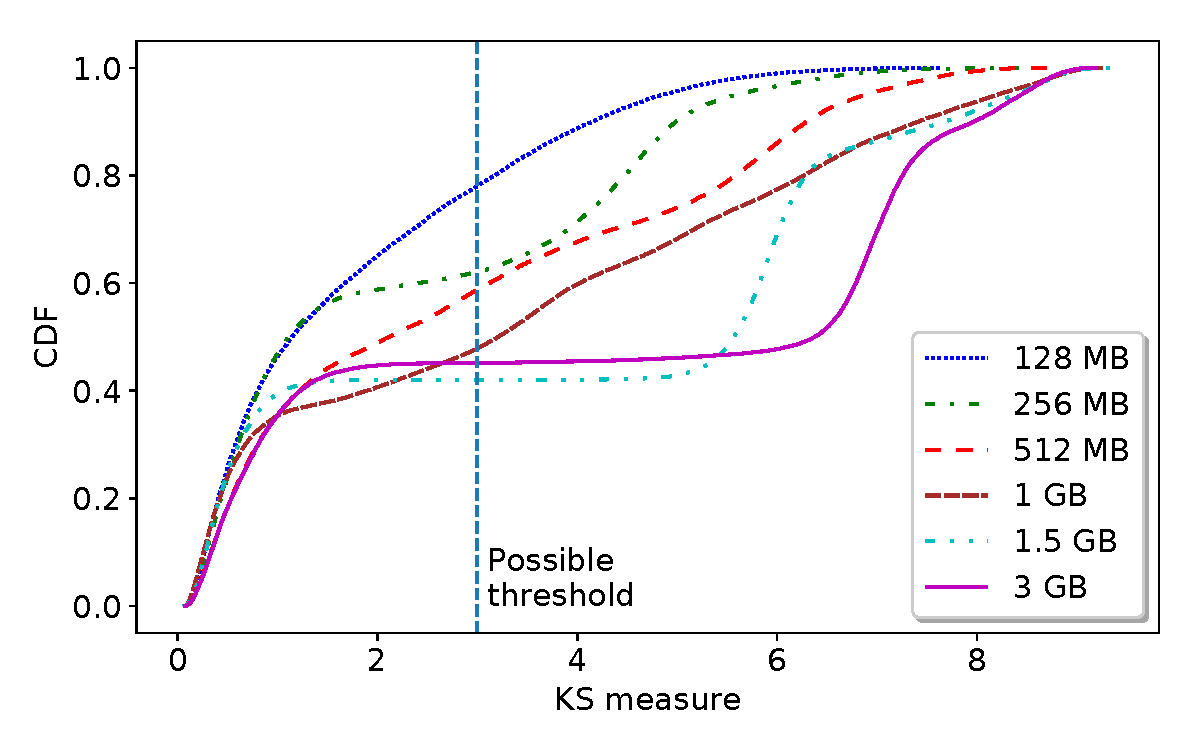
\includegraphics[width=.99\linewidth]{fig/ksvalues.pdf}
  \caption{We present a CDF of KS values observed for various lambda sizes. A bimodal distribution 
  with a longer step allows us to pick a KS-threshold that enables our technique to differentiate 
  between 0-bit and 1-bit with high confidence. 
\label{fig:ks_values}}
\end{figure}


